% topic1.tex -- Module 8 Topic 1: Origins of the elements, Q1-14.
\firsttopictitle{Topic 1 - Origins of the Elements}

% ---- Q1 (order of events after the Big Bang)
\begin{quizq}{}
Which list shows the order in which these first formed after the Big Bang?
\opts{Neutral atoms, light nuclei, protons and neutrons, quarks}
  {Light nuclei, quarks, neutral atoms, protons and neutrons}
  {Quarks, protons and neutrons, light nuclei, neutral atoms}
  {Protons and neutrons, quarks, neutral atoms, light nuclei}
\end{quizq}

% ---- Q2 (evidence for the Big Bang)
\Needspace{15\baselineskip}
\begin{quizq}{}
Which observation is evidence for the Big Bang theory?
\opts{Microwave radiation with a black-body spectrum (about \qty{2.7}{K}) comes almost equally from every
   direction in space.}
  {Most stars lie on the main sequence of the Hertzsprung--Russell diagram.}
  {The spectrum of the Sun contains dark absorption lines.}
  {The planets orbit the Sun in elliptical paths.}
\end{quizq}

% ---- Q3 (Hubble's law graph)
\Needspace{30\baselineskip}
\begin{quizq}{}
Which graph best shows the relationship that Hubble found between the recession velocity $v$ of
galaxies and their distance $d$ from Earth?
\gridopts{%
  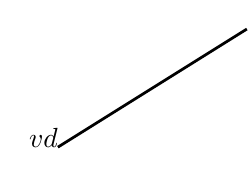
\begin{tikzpicture}\gaxesP{$v$}{$d$}
    \draw[line width=1pt] (0,0) -- (2.4,1.5);
  \end{tikzpicture}}
  {%
  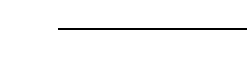
\begin{tikzpicture}\gaxesP{$v$}{$d$}
    \draw[line width=1pt] (0,1.0) -- (2.4,1.0);
  \end{tikzpicture}}
  {%
  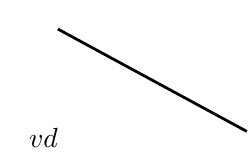
\begin{tikzpicture}\gaxesP{$v$}{$d$}
    \draw[line width=1pt] (0,1.5) -- (2.4,0.2);
  \end{tikzpicture}}
  {%
  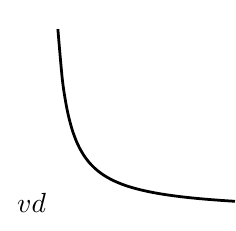
\begin{tikzpicture}\gaxesP{$v$}{$d$}
    \draw[line width=1pt, domain=0.15:2.4, samples=40, smooth] plot (\x, {0.35/\x});
  \end{tikzpicture}}
\end{quizq}

% ---- Q4 (Hubble constant)
\Needspace{12\baselineskip}
\begin{quizq}{}
A galaxy \qty{120}{Mpc} from Earth is moving away at \qty{8400}{km.s^{-1}}. What value of the Hubble
constant does this give, in \si{km.s^{-1}.Mpc^{-1}}?
\opts{0.014}{70}{\num{8.4e3}}{\num{1.0e6}}
\end{quizq}

% ---- Q5 (age of the universe from 1/H0)
\Needspace{14\baselineskip}
\begin{quizq}{}
The Hubble constant is \qty{70}{km.s^{-1}.Mpc^{-1}}, where $\qty{1}{Mpc} = \qty{3.09e22}{m}$. Using
$t = \dfrac{1}{H_0}$ and $\qty{1}{year} = \qty{3.16e7}{s}$, what is the approximate age of the universe?
\opts{\qty{4.4e17}{years}}{\qty{1.4e13}{years}}{\qty{1.4e10}{years}}{\qty{1.4e7}{years}}
\end{quizq}

% ---- Q6 (HR diagram: identify a red giant and a white dwarf)
% W upper right (red giant), X lower left (white dwarf), Y upper left and Z lower right (main sequence)
\Needspace{36\baselineskip}
\begin{quizq}{}
The Hertzsprung--Russell diagram shows four stars, W, X, Y and Z.
\begin{center}
  \begin{tikzpicture}[x=1cm, y=0.5cm]
    \draw[line width=0.7pt] (0,0) -- (6.4,0) node[right, font=\small, align=left] {Surface\\temperature};
    \draw[axisline] (0,0) -- (0,8.6) node[above, font=\small] {Luminosity (Sun $= 1$)};
    \foreach \y/\l in {1/$10^{-4}$, 3/$10^{-2}$, 5/$1$, 7/$10^{2}$} {\draw (0,\y) -- (-0.08,\y) node[left, font=\scriptsize] {\l};}
    \foreach \x/\l in {0.5/\qty{30000}{K}, 3/\qty{10000}{K}, 5.5/\qty{3000}{K}} {\draw (\x,0) -- (\x,-0.15) node[below, font=\scriptsize] {\l};}
    \draw[line width=6pt, black!15, line cap=round, smooth] plot coordinates {(0.6,8.4) (2.0,7.6) (3.2,6.5) (4.16,5.0) (4.9,3.4) (5.6,1.6)};
    \node[font=\scriptsize, black!60, rotate=-22] at (2.6,7.55) {main sequence};
    \fill (5.0,6.8) circle (2.5pt) node[right, font=\small] {W};
    \fill (1.2,3.0) circle (2.5pt) node[right, font=\small] {X};
    \fill (1.0,8.15) circle (2.5pt) node[right, font=\small] {Y};
    \fill (5.2,2.6) circle (2.5pt) node[right, font=\small] {Z};
  \end{tikzpicture}
\end{center}
Which row correctly identifies a red giant and a white dwarf?
\begin{center}
  \renewcommand\arraystretch{1.7}
  \begin{tabular}{@{}p{10mm}|>{\centering\arraybackslash}p{40mm}|>{\centering\arraybackslash}p{40mm}|}
    \cline{2-3}
    & \textit{Red giant} & \textit{White dwarf}\\ \cline{2-3}
    A. & Y & Z\\ \cline{2-3}
    B. & Z & X\\ \cline{2-3}
    C. & X & W\\ \cline{2-3}
    D. & W & X\\ \cline{2-3}
  \end{tabular}
\end{center}
\end{quizq}

% ---- Q7 (cluster ages from the turn-off point)
\Needspace{16\baselineskip}
\begin{quizq}{}
The HR diagrams of three star clusters are compared. In cluster P, the main sequence still includes
hot blue O and B stars. In cluster Q, the main sequence ends at A stars. In cluster R, it ends at
Sun-like G stars. Which list orders the clusters from youngest to oldest?
\opts{P, Q, R}{R, Q, P}{Q, P, R}{P, R, Q}
\end{quizq}

% ---- Q8 (what stars in a globular cluster share)
\Needspace{12\baselineskip}
\begin{quizq}{}
The stars in a globular cluster are often plotted together on one HR diagram. Which property do the
stars in the cluster share?
\opts{The same mass}{About the same age}{The same luminosity}{The same surface temperature}
\end{quizq}

% ---- Q9 (same spectral class, different luminosity)
\Needspace{15\baselineskip}
\begin{quizq}{}
Stars P and Q have the same spectral class, but star P has 100 times the luminosity of star Q. What is
the best explanation?
\opts{Star P is hotter than star Q.}{Star P is closer to Earth than star Q.}
  {Star P has a much larger radius than star Q.}{Star P is younger than star Q.}
\end{quizq}

% ---- Q10 (proton-proton chain)
\Needspace{12\baselineskip}
\begin{quizq}{}
In one step of the proton--proton chain, a deuterium nucleus (\nuc{2}{1}{H}) fuses with a proton. Which
nucleus is formed?
\opts{\nuc{4}{2}{He}}{\nuc{3}{1}{H}}{\nuc{2}{2}{He}}{\nuc{3}{2}{He}}
\end{quizq}

% ---- Q11 (CNO cycle)
\Needspace{14\baselineskip}
\begin{quizq}{}
In which stars is the CNO cycle the main source of energy?
\opts{In all stars}{Main-sequence stars more than about 1.3 times the mass of the Sun}{Red dwarf stars less massive than the
  Sun}{White dwarf stars}
\end{quizq}

% ---- Q12 (energy from the proton-proton chain)
\Needspace{12\baselineskip}
\begin{quizq}{}
In the proton--proton chain, the total mass of the products is \qty{0.0287}{u} less than the mass of
the particles that react. How much energy is released?
\opts{\qty{3.0e-16}{MeV}}{\qty{4.3e-12}{MeV}}{\qty{0.0287}{MeV}}{\qty{26.7}{MeV}}
\end{quizq}

% ---- Q13 (massive main-sequence star compared with the Sun)
\Needspace{20\baselineskip}
\begin{quizq}{}
A main-sequence star has 10 times the mass of the Sun. Which row correctly compares it with the Sun?
\begin{center}
  \renewcommand\arraystretch{1.7}
  \begin{tabular}{@{}p{10mm}|>{\centering\arraybackslash}p{45mm}|>{\centering\arraybackslash}p{45mm}|}
    \cline{2-3}
    & \textit{Luminosity} & \textit{Time on the main sequence}\\ \cline{2-3}
    A. & Higher & Shorter\\ \cline{2-3}
    B. & Higher & Longer\\ \cline{2-3}
    C. & Lower & Shorter\\ \cline{2-3}
    D. & Lower & Longer\\ \cline{2-3}
  \end{tabular}
\end{center}
\end{quizq}

% ---- Q14 (elements heavier than iron)
\Needspace{15\baselineskip}
\begin{quizq}{}
How are elements heavier than iron produced?
\opts{By fusion in the core of the Sun}{By fusion in the cores of massive stars, which releases energy}
  {Mainly by neutron capture, in red giant stars, supernovae and neutron-star mergers}
  {By nuclear reactions in the first few minutes after the Big Bang}
\end{quizq}
